\chapter{Background} %\label{1cap:spinta_laterale}
% [titolo ridotto se non ci dovesse stare] {titolo completo}

Al giorno d'oggi è sempre più frequente adottare soluzioni che facciano uso di moduli intelligenti all'interno dei più svariati ambiti lavorativi, ed è oramai risaputo come tali soluzioni debbano rispettare tutta una serie di standard qualitativi, affinché possano essere ritenuti attendibili ai loro scopi. Tuttavia recenti studi hanno dimostrato un nuova gamma di difetti che evidenziano una serie di vulnerabilità, fin ora non riscontrate all'interno dello sviluppo software (tra cui, come verrà approfondito in seguito in questo capitolo, quelle dovute alla la Software Fairness), legati all'operare in maniera imparziale ed equa nel loro contesto di utilizzo \cite{brun2018software}. Per capire come il mondo dello sviluppo software (ed in particolare quello delle soluzioni "intelligenti"), siano influenzati dagli aspetti di equità o un qualsiasi altro aspetto qualitativo in generale è doveroso introdurre gli aspetti essenziali che si pongono alla base dello sviluppo di tali applicativi.

\section{Ingegneria del Software}
Prima di tutto è senz'altro necessario far riferimento all'ingegneria del Software, disciplina che nasce proprio in risposta alle problematiche di sviluppo di prodotti software di qualità in un preciso tempo, con uno specifico budget \cite{Bruegge2009ObjectOrientedSE}. L'ingegneria del Software si pone l'obiettivo di applicare tutta una serie di attività che facciano dello sviluppo software un vero e proprio processo ingegneristico \cite{mall2018fundamentals}.  Le attività cardine della materia, cosi come definite da Bernd Bruegge e Allen Dutoit, \cite{Bruegge2009ObjectOrientedSE}, sono:

\begin{itemize}
    \item La \emph{modellazione}: capacità standard di focalizzarsi sui dettagli rilevanti ignorando tutto il resto, tramite svariate strategie di raffinamento e astrazione;
    \item Il \emph{problem solving}: l'utilizzo di modelli per la ricerca di soluzioni a specifici problemi;
    \item L' \emph{acquisizione di conoscenza}: la raccolta di singoli dati e informazioni di uno specifico dominio, per poi formularne informazioni e conoscenza prima di applicare standard di sviluppo;
    \item La \emph{ricerca di un razionale}: cioè la ricerca delle motivazioni e delle necessità che si pongono a priori dello sviluppo di un tool software;
\end{itemize}

Si osserva quindi come effettivamente un tool software per essere progettato in maniera congrua a molteplici aspetti qualitativi - ad esempio: sicurezza, manutenibilità e adattabilità (o qual si voglia tipologia di attributo non funzionale) - che soddisfino le aspettative del cliente che lo commissiona, sia necessario applicare un processo standard di ingegnerizzazione. Nello specifico, anche problematiche legate all'emergente tematica dell'equità e dei vincoli di imparzialità devono essere trattati sullo stesso piano di un qualsiasi altro attributo qualitativo e la ricerca si sta muovendo sempre di più in questa direzione \cite{brun2018software}.

Ovviamente, è molto complesso cercare di riassumere in poche parole ogni peculiarità dell'ingegneria del software, molteplici sono gli aspetti di disciplina che caratterizzano un prodotto software, e.g. il suo ciclo di vita, la sua manutenzione ed evoluzione, e tutti gli aspetti correlati alla sua gestione. Lo stesso testo di riferimento \cite{Bruegge2009ObjectOrientedSE}, definisce l'ingegneria del software, come un attività complessa, non come un algoritmo standard, quindi è importante osservare come essa si adatti in maniera dinamica, agli specifici problemi, e a seconda dei casi faccia uso in maniera oculata di strumenti di vario tipo, come la sperimentazione e la misurazione, il riuso di pattern o l'evoluzione incrementale dei sistemi \cite{Bruegge2009ObjectOrientedSE} e altre variegate tecniche e metodologie che possano offrire pronta risposta alla più ampia gamma di problematiche e necessità specifiche. Volendo porre un esempio più specifico di come l'ingegneria del software vada a specializzarsi nei contesti specifici di sviluppo, è possibile far riferimento all'ampiamente utilizzato sviluppo software Object-Oriented, che specializza un \emph{tradizionale} ciclo di sviluppo software in sei attività di sviluppo \cite{Bruegge2009ObjectOrientedSE}: 

\begin{itemize}
    \item  \emph{Raccolta e Analisi dei requisiti}, grazie alle quali gli ingegneri del software, analizzano il problema con il cliente al fine di definire, i confini del dominio applicativo;
    \item \emph{System Design}, fase in cui gli ingegneri del software analizzano il problema e lo dividono in piccoli pezzi, al fine di selezionare strategie generali di design per il problema proposto;
    \item l'\emph{Object Design}, fase in cui vengono selezionate soluzioni dettagliate per ogni \emph{sotto-problema};
    \item l'\emph{Implementazione del sistema}, che corrisponde solo ad uno degli ultimi passi del ciclo di sviluppo, durante la quale gli sviluppatori \emph{traducono} la soluzione al problema in codice sorgente;
    \item Il \emph{Testing}, fase in cui gli sviluppatori cercano differenze tra il sistema implementato e i suoi modelli sulla base di ben definiti campioni di dati di input.
\end{itemize}

Come osservato, l'ingegneria del software, offre anche tutta una serie di attività gestionali che interessano ed influenzano un canonico progetto software.  Le attività di gestione si focalizzano sulla pianificazione di un progetto software, il monitoraggio del suo status di avanzamento, il tracciamento dei suoi cambiamenti e la coordinazione delle risorse, al fine di consegnare un prodotto di alta qualità in relazione a quelli che sono i vincoli a cui esso è soggetto, come ad esempio quelli di tempo e di costo \cite{Bruegge2009ObjectOrientedSE}. \\

Altra branca dell'ingegneria del software, che da attività finale di un canonico modello ciclo di vita del software è diventa un processo a se stante che caratterizza l'evoluzione del prodotto per tutta la sua durata di vita è la \emph{manutenzione}, macro-processo che include tutte quelle attività che occorrono dopo la consegna del sistema al cliente. La manutenzione è un aspetto complesso, ma sempre più necessario al fine di garantire il successo dei sistemi software, sempre più orientati al cambiamento \cite{Bruegge2009ObjectOrientedSE}. Basti pensare che già nel 1974, uno dei più noti studiosi del campo Henry Lehman, osservava l'importanza dell'evoluzione e della manutenzione, con la formulazione delle prime leggi sull'evoluzione del software. Le leggi di Lehman, sono ancora oggi dei principi cardine degli studi sull'evoluzione del software, e se si pensa anche solo alle prime due, si intuisce l'importanza del processo di manutenzione \cite{SEMaintenance} :

\begin{itemize}
    \item \emph{Prima Legge di Lehman}: I programmi di tipo evolutivo, devono necessariamente essere adattati \emph{al cambiamento}, altrimenti essi diventano progressivamente meno soddisfacenti;
    \item \emph{Seconda Legge di Lehman}: Così come un programma (sistema software) evolve, così la sua complessità aumenta, a meno che del lavoro non venga fatto al fine di manutenerla e ridurla.
\end{itemize}

Per concludere, in maniera opportuna l'introduzione all'ingegneria del software è doveroso far riferimento alle metodologie agili e allo sviluppo incrementale, che nel corso degli ultimi decenni stanno prendendo sempre più piede nel contesto ingegneristico. Secondo le più note fonti presenti in letteratura, questa tipologia di approcci e metodologie, sono caratterizzati da alcuni principi innovativi che si discostano quasi del tutto dall'idea di ciclo di sviluppo tradizionale. Ian Sommerville, nel suo volume \emph{Software Engineering}, riassume il core dei processi agili, facendo riferimento alle seguenti caratteristiche\cite{Sommerville10}:

\begin{itemize}
    \item Il rilascio di nuove release dei sistemi caratterizzate da piccoli cambiamenti ogni due o tre settimane circa; 
    \item Il coinvolgimento continuo dei clienti al fine di ottenere rapidi feedback e tracciare i continui cambiamenti;
    \item La riduzione della  documentazione, \emph{al minimo indispensabile}, preferendo l'uso di comunicazioni informali, piuttosto che meeting formali con documenti scritti;
    
\end{itemize}
\section{Intelligenza Artificiale e Machine Learining}
L'Intelligenza Artificiale ed in particolare i moduli di Machine Learning, stanno diventando sempre di più una parte fondamentale delle applicazioni commerciali e dei progetti di ricerca nell'ambito IT. In particolare si osserva come i moduli addestrati di maggior successo, siano realizzate a partire dalla generalizzazione di esempi noti (basi di conoscenza), sulle quali i moduli stessi vengono addestrati, al fine di produrre, sulla base di dati di input forniti, un output desiderato senza che l'utente umano dia informazioni aggiuntive. La branca del Machine Learning, nella quale vengono racchiusi tutti gli algoritmi che si basano su tali tuple di \textit{input-output} viene definita come \textbf{Apprendimento Supervisionato} \cite{libroMLs}.
Dalla stessa fonte possiamo osservare come esempi di apprendimento supervisionato di interesse possano essere:
\begin{itemize}
    \item L'identificazione di \textit{topix} da un blog o un sito internet;
    \item l'identificazione di pattern di accesso anomali in un sito web;
    \item la suddivisione dei clienti di uno shop per preferenze similari.
\end{itemize}

Soprattutto negli ultimi anni, si ci sta accorgendo che l'applicazione combinata di discipline come la statistica, la teoria dell'informazione e il machine learning, stanno portando alla creazione di una scienza sempre più solida, con una ferma base matematica, e a tool sempre più potenti. In particolare, se si fa riferimento al learning supervisionato tecniche e algoritmi come alberi di decisione, regressione lineare, regressione logistica, clustering, sono alcune delle tecniche più utilizzate per la progettazione di componenti AI, per innumerevoli campi applicativi, ed in particolare quello che ne risulta dall'applicazione di una generica tecnica di learning supervisionato, su un dataset di addestramento, è definito come processo di classificazione \cite{supervisedML&Classification}. \\

Per capire praticamente la problematica di classificazione in ambito machine learning, si può pensare di far riferimento al comune esempio di identificazione delle mail di spam, tecnica automatica di filtering basata su di grandi data set ampiamente utilizzata dai gestori di mailing. In pratica, sulla base dei dati (strutturali, storici e similari) a disposizione di mail già contrassegnate o meno come "SPAM" è possibile addestrare un modello, al fine di classificare una nuova mail che un generico utente riceve come "SPAM MAIL" oppure "NON SPAM MAIL". Volendo dare quindi una definizione semi formale: il problema di classificazione del Machine Learning consiste nell'\textit{individuare una \textbf{categoria} (ad esempio MAIL di SPAM oppure MAIL NON DI SPAM) per una \textbf{nuova osservazione} (e.g. una nuova mail ricevuta), sulla base di precedenti \textbf{dati di addestramento} contenenti informazioni già classificati secondo \textbf{categorie note} (ad esempio archivio di mail già classificate come SPAM oppure NON SPAM a disposizione del modulo addestrato}".\\

Questa problematica è particolarmente attenzionata dalla ricerca, dato che è molto complesso generare classificatori che non soffrano di alcuni problemi noti in letteratura, come ad esempio, la stretta dipendenza dal dataset di partenza \cite{supervisedML&Classification}, il così detto fenomeno del \textit{garbage-in,garbage-out}, cioè la presenza di Bias nei dataset di addestramento, che poi tenderanno a riflettersi all'interno delle predizione dei moduli di previsione stessi \cite{evalFairClassification}. Volendo porre un esempio pratico, nell'ambito dell'etica del software, è facile che un classificatore addestrato con un dataset, non immune a dei bias su specifici attributi sensibili (quali razza o sesso), possa essere addestrato in modo tale da effettuare predizioni imparziali, spesso rivolte a favore degli individui del campione di addestramento dei gruppi di maggioranza (ovvero quegli individui che posseggono il valore più ricorrente dell'attributo sensibile) \cite{evalFairClassification} .


\subsection{Algoritmi di ricerca e Algoritmi Genetici}
Il machine learning è sicuramente uno degli aspetti più caratterizzanti dell'intelligenza artificiale, al fine di fornirne una panoramica più ampia è interessare considerare anche gli algoritmi di ricerca. Essi per definizione sono usati per restituire informazioni memorizzate all'interno di strutture dati o ricercare soluzioni in un complesso spazio di ricerca formalmente definito sulla base del dominio del problema, il tipo di informazioni gestite dagli algoritmi di ricerca possono essere formate da valori discreti e continui. Di algoritmi di ricerca ne esistono in letteratura di vari tipi, basati su vari approcci: algoritmi basati sull'uso di una funzione di costo (e.g. depth-first, bread-first e cost-uniform first...), basati sull'utilizzo di euristiche (e.g. A* greedy best-first), algoritmi di ricerca locale (e.g. hill-climbing search) ecc., ma tra i più usati in ambito di ricerca ci sono sicuramente gli algoritmi di tipo evolutivo ed in particolare quelli di tipo genetico. Gli algoritmi genetici, sono algoritmi basati sui principi della selezione naturale e della genetica, introdotti negli anni '70  da J.Holland e ispirati alle teorie dell'evoluzione degli esseri viventi \cite{geneticalgotihm}. Gli algoritmi genetici astraggono lo spazio del problema come una popolazione di individui, e provano ad esplorare le caratteristiche degli individui, "producendone" di nuovi in maniera iterativa. I GA evolvono la popolazione da individui iniziali (spesso generati casualmente) in individui di alta qualità, laddove ogni individuo rappresenta una soluzione al problema di interesse codificata in stringa. La qualità di ogni individuo è misurata da una funzione matematica detta funzione di fitness che è formulata in modo tale da valutare in maniera quantitativa la bontà di un individuo, a seconda di alcune caratteristiche qualitative definite dallo sviluppatore. A seconda del problema la funzione di fitness, può essere di massimizzazione, di minimizzazione, a singolo obiettivo o multi obiettivo, e spesso rappresenta l'ostacolo più grande nella progettazione di un algoritmo genetico. \\

Durante ogni generazione, tre operatori di base della genetica sono applicati in sequenza con una certa probabilità: selezione, crossover e mutazione \cite{geneticalgotihm} . I passaggi base di un algoritmo di ricerca genetico sono:
\begin{enumerate}
    \item Generazione randomica di una popolazione di n individui (rappresentanti di soluzioni randomiche al problema);
    \item Valutazione di ogni individui tramite la funzione di fitness;
    \item Selezione di due individui per generarne di nuovi (nuova generazione), le tecniche di selezione possono essere diverse, tra le più famose ci sono: la roulette wheel e l'approccio a torneo;
    \item Con una certa probabilità, viene applicata un operazione di cross over al fine di mischiare singole parti degli individui selezionati per generarne di nuovi (anche qui ne esistono vari tipi). Se il crossover non viene applicato, in sostituzione vengono copiati "i genitori";
    \item Con una certa  probabilità ai nuovi individui vengono applicate operazioni di mutazione (ovvero vengono cambiati uno o più dati della stringa casualmente);
    \item Gli individui generati, vengono aggiunti alla popolazione, al fine di far ripartire l'algoritmo;
    \item Se uno degli individui generati soddisfa le condizioni di accettazione e di arresto dell'algoritmo, allora si ritorna la soluzione migliore trovata fino a quel momento;
    \item Altrimenti l'algoritmo riparte dal passo 2;
    
\end{enumerate}


\section{Ingegneria del Software nell'Intelligenza artificiale}

Si può osservare come negli ultimi decenni, l'intelligenza artificiale e l'ingegneria del software, si siano evolute separatamente, oggi giorno, si osserva però come la ricerca attuale, stia portando alla specifica e alla costituzione di nuovi studi e approcci allo sviluppo di soluzioni AI-Intensive, che tengano proprio conto dell'intersezione che c'è tra l'ingegneria del software e l'intelligenza artificiale \cite{rech2004artificial}. L'Intelligenza artificiale odierna fa riferimento a sistemi che sulla base degli input che ricevono in considerazione devono assumere rischi, fare predizioni o assumere comportamenti in risposta a specifici problemi \cite{shaw2019artificial}, in dettaglio, nell'era dei computer dalle elevate prestazioni e dei Big Data, molte soluzioni AI-Intensive, sono sviluppate in risposta ai bisogni che la quotidianità sociale necessita, ma come noto in letteratura, molti sistemi software di grandi dimensioni, non sono privi di bug, ed in particolare i sistemi di Intelligenza Artificiale e di Machine Learning non fanno eccezione. Per questa tipologia di sistemi, bug di progettazione o addestramento, possono essere causa di crush di sistema, output errati fino all'esecuzione troppo lenta che non rende possibile l'utilizzo di tali soluzioni nell'ambiente di lavoro \cite{ML&Bugs}. In casi critici gli errori dei sistemi intelligenti, possono addirittura portare alla morte di chi anche involontariamente interagisce con essi, il caso più noto è quello della ciclista Elaine Herzberg, morta investita da un'auto con pilota automatico, per errore di valutazione del modulo di guida \cite{shaw2019artificial}. Quindi come è possibile produrre soluzioni AI Intensive per il mondo reale, che tengano conto di tali problematiche? L'applicazione dell'ingegneria del software cerca in qualche modo di dare risposta a questa tipologia di problematica, in dettaglio, si cerca di includere metodi di Requirement Engineering, Design Engineering, Code Engineering e Project Management, che possono essere di supporto, per lo sviluppo di Sistemi Ai-Intensive efficienti. La ricerca stessa ne fa utilizzo, ed infatti molti ambiti di studio sono nati dall'intersezione tra SE e AI, in particolare vale la pena citare l'Agent Oriented Software Engineering oppure l'Ambient Intelligence \cite{jain2011interaction}. L'Agent Oriented Software Engineering, si concentra sullo sviluppo di soluzioni che siano, intelligenti, agili e pro-attive. In dettaglio il suo scopo principale è quello di sviluppare soluzioni AI-intensive tramite dei riadattamenti stessi delle tecniche di Ingegneria del Software, per lo sviluppo di Agenti di piccoli e grandi dimensioni. Nel dettaglio risultano essere di rilievo l' \textit{Agent UML}, per la progettazione dei moduli agente, oppure metodi di specifica e valutazione formali dei sistemi, i quali hanno lo scopo intrinseco di validare gli obiettivi, i comportamenti di un singolo agente, e soprattutto le interazioni nei sistemi multi agente \cite{rech2004artificial}. l'Ambient Intelligence invece si pone lo scopo di progettare ambienti di addestramento (secondo tecniche specifiche dell'ingegneria del software) che siano sensibili ed adattabili agli stimoli esterni e in conseguenza, sistemi reattivi che siano informati circa i bisogni, le abitudini e le emozioni degli utenti per supportare il loro lavoro quotidiano\cite{rech2004artificial}.\\

Qualsiasi branca o studio di ricerca a cui si voglia far riferimento (come gli esempi riportati) definita nella così detta "intersezione tra intelligenza artificiale e ingegneria del software", non può prescindere dall'analizzare quelli che sono i requisiti non funzionali di qualità che una soluzione AI-Intensive deve rispettare. In particolare in letteratura \cite{NFRForML}, si può osservare come, ad esempio, il Machine Learning sia soggetto a specifici vincoli di qualità quali: 

\begin{itemize}
    \item \emph{Accuracy and Performances}, come l'output di un agente risulta "corretto" se paragonato alla realtà;
    \item \emph{Fairness}, Requisito che si pone l'obiettivo di rendere gli algoritmi di ML più \textbf{imparziali} e indipendenti da bias di dati;
    \item \emph{Transparency}, ovvero la capacità di dimostrare come i risultati elaborati da un modulo intelligente siano affidabili e trasparenti, ricostruendo le fonti di partenza;
    \item \emph{Security and Privacy}, \emph{Testability} e \emph{Reliability} del modulo addestrato.
\end{itemize}

Per progettare, realizzare e controllare questi aspetti qualitativi essenziali per un modulo di intelligenza artificiale, la ricerca è enormemente incentrata nello studio di questi aspetti. In particolare, si nota come questi requisiti non funzionali, siano particolarmente attenzionati dall'ingegneria dei requisiti, branca dell'ingegneria del software che si incentra nella specifica, l'analisi, la verifica e la validazione dei requisiti di un sistema software \cite{RE&Ai}, la cui ricerca ricerca sta incentrando buona parte dell'effort nello studio di aspetti quali fairness, privacy, sostenibilità e modificabilità anche per tecniche di Machine Learning e per lo sviluppo di soluzioni AI-Intensive in generale \cite{NFRForML}. In particolare, la letteratura afferma come l'industria dell'intelligenza artificiale è particolarmente incentrata nello sviluppo di soluzioni di Machine Learning e basate sugli approcci Data Driven, ed una delle principali aree di interesse per lo sviluppo di questo tipo di soluzione è il settore dell'Healthcare, particolarmente caratterizzato dalla mancanza di standard di progettazione e dalla continua evoluzione dei dati a disposizione\cite{RE&Ai}, per far fronte a questa tipologia di problematiche, l'ingegneria del software ed in particolare l'ingegneria dei requisiti, pongono l'accento su nuove metodologie e tecniche che toccano vari processi di un sistema AI-Intensive: la specifica e l'analisi dei suoi requisiti, la validazione del modello (e quindi delle sue specifiche), la documentazione e il management dell'intero processo di sviluppo dei requisiti formulati. Le sfide principali che la ricerca ha davanti in quella che è stata definita \textit{intersezione} tra intelligenza artificiale e ingegneria del software sono:

\begin{itemize}
    \item \emph{Lo Skill Gap}: la necessità di creare lo giusto spirito di collaborazione aziendale tra Data Scientist e Ingegneri del Software;
    \item \emph{Il Data Gap}: Ovvero la necessità di rendere disponibili (big) dataset necessari alla realizzazione di soluzioni AI complesse;
    \item \emph{L'Engeeniring Gap}, ovvero la necessità di creare prototipi generalizzabili dei sistemi AI, con il giusto supporto all'intero ciclo di vita della Soluzione AI-Intensive;
\end{itemize}


\subsection{Machine Learning Life Cicle e ML Pipeline}
Uno dei contributi generali che l'ingegneria del software cerca di dare all'intelligenza artificiale è proprio quello di sistematizzare la progettazione e lo sviluppo dei suoi modelli. In tal senso lo sviluppo di una soluzione AI-Intensive, così come un generico progetto di Machine Learning, può essere sistematizzato definendo opportuni processi ingegneristici e di conseguenza un vero e proprio ciclo di vita della soluzione che si sta progettando. Ogni progetto AI-Intensive, quindi può avere uno specifico ciclo di vita, e concentrandosi nel del machine learning, Burkov e Andriy affermano che un progetto ML-Intensive è caratterizzato inizialmente dalla comprensione e dall'analisi dello scope applicativo e degli obiettivi di business il modello \cite{burkov2020machine}, successivamente il primo passo che porta alla nascita di un modello di machine learning è capire se il modello stesso ha dei precisi obiettivi. Gli obiettivi di un modello ML-Intensive sono ovviamente diversi da quelli di business e dettano le basi di progettazione del modello stesso, un generale obiettivo di un modello ML, deve essere formalizzato in modo tale da tener conto \cite{burkov2020machine}:

\begin{enumerate}
    \item Di cosa il modello riceve come input;
    \item Di cosa genera come output;
    \item Dei criteri di accettabilità (o inaccettabilità) del comportamento del modello;
\end{enumerate}

Il ciclo di vita di un modello di machine learning può essere sistematizzato tramite i seguenti passaggi \cite{burkov2020machine}:

\begin{enumerate}
    \item Definizione degli obiettivi;
    \item Collezione e preparazione dei dati;
    \item Ingegnerizzazione delle feature;
    \item Training del modello;
    \item Evoluzione del Modello;
    \item Deployment del Modello;
    \item Fase operativa del modello e monitoraggio;
    \item Manutenzione del modello.
\end{enumerate}

Approcci più innovativi allo sviluppo ML-Intensive, sottolineano come aspetti di monitoraggio, architecturing e monitoring continuo, siano essenziali per far evolvere un modello di pari passo con il suo ambiente di utilizzo, uno degli approcci innovativi che cerca di rispondere a queste esigenze è la specializzazione ML di DevOps, che appunto prende il nome di MLOps.\\

I passaggi del ciclo di vita di vita di un modello ML-Intensive, possono essere anche organizzati e automatizzati in modo tale da configurare una vera e propria \textbf{pipeline di machine learning}, che viene definita come una sequenza di operazioni su un dataset che vanno dal suo stato iniziale, fino al rilascio del modello e la sua evoluzione. Una pipeline può includere tra i passaggi di preparazione dei dati, imputation dei dati mancanti, estrazione delle feature, data augmentation e model training\cite{burkov2020machine}. In pratica, una delle innovazioni più forti portati dalla formalizzazione di una pipeline di machine learning, è che quando un modello di machine learning è deployato in produzione, in realtà è deployata l'intera pipeline\cite{burkov2020machine} (rispondendo in maniera \emph{automatizzata} alle necessità evolutive del modello. Da notare che una pipeline di machine learning è generalmente ottimizzata quando i suoi hyperparameters di configurazione sono ottimizzati (Hyperparameters tuning) \cite{burkov2020machine}.

\subsection{Piattaforme per Machine Learning Pipelines e MLOps}
Dare la definizione di Machine Learning Pipeline, fa capire come lo sviluppo e il deploying di applicazioni ML-Intensive, è un processo che va ben oltre i dati collezionati e i modelli addestrati e fare predizioni. Come osservato da Zhou et al. connettere queste parti ignorando la fase di manutenzione del modello, costituisce un enorme debito tecnico \cite{MLOps}. Costruire un workflow dal data pre-processing fino al porre il modello in run nel contesto di utilizzo, può facilmente essere un processo dispendioso in termini di tempo e soprattutto non privo di errori, tra l'altro una produzione efficiente e affidabile è fondamentalmente critico per molti contesti reali, si pensi a casi d'uso quali la guida automatica oppure l'health care\cite{MLOps}. \\

In risposta a queste esigenze critiche, sono nate piattaforme di machine learning, che in maniera embedded forniscono un ciclo di vita manageriale end-to-end per applicazioni ML-Intensive, core primario di queste applicazioni cercano di accorpare sistemi stand-alone che in maniera specificano si assumono responsabilità di task quali: data-preprocessing, model training, model evolution e messa in servizio. Goal primario di queste piattaforme è quello fornire una soluzione generica per molteplici casi d'uso di sviluppo, collegando e configurando componenti indipendenti per specifiche problematiche. Con questa tipologia di configurazione, un generico workflow ML può essere orchestrato e convertito in una vera e propria Pipeline di Machine Learning, la cui esecuzione è supportata da queste piattaforme \cite{MLOps}. Oltretutto il livello di affidabilità, scalabilità, abilità di continuous training, fornito da questi strumenti, offre la possibilità di adattare e ed evolvere i dati oppure incrementare i cambiamenti frequentemente \cite{MLOps}.\\

Con la creazione di Tools che permettono di ingegnerizzare una pipeline di machine learning, hanno portato nell'ambito dell'ingegneria del software alla nascita di vere e proprie culture e pratiche di sviluppo specifiche. la più nota nel mondo dell'intelligenza artificiale è sicuramente \emph{MLOps}, che specializza nell'ambito AI, la più generica cultura di sviluppo software \emph{DevOps}. 

Per comprendere bene un processo di sviluppo ML-intensive, basato sulla filosofia ML-Ops, è necessario comprendere innanzitutto, quali sono i processi generali che entrano in gioco durante il ciclo di vita di una soluzione ML-Intensive. Innanzitutto è necessario distinguere quelli che sono i processi di sviluppo, che racchiudono \cite{MLOpsBook}:

\begin{itemize}
    \item Raccolta e manipolazione dei dati grezzi;
    \item Analisi e processing dei dati per il training;
    \item Costruzione, training e testing del modello;
    \item Overfitting e tuning del modello;
    \item Validazione del modello.
    
\end{itemize}

da quelli che vengono invece definiti processi derivanti dall'uso del modello nell'ambiente di utilizzo, chiamati appunto processi operazionali eseguiti da figure professionali dedicate, in particolare possono essere definiti processi operazionali per una soluzione ML-Intensive \cite{MLOpsBook}:

\begin{itemize}
    \item Deployment del modello;
    \item Monitoring del modello;
    \item Formulazione di statistiche di reporting;
    \item Feedback retrival al team di manutenzione;
\end{itemize}

DevOps, o development operations, è una cultura più generale di sviluppo ingegneristica, che si riferisce a set di pratiche che combinano i generici processi di sviluppo software, con quelli operazionali, in modo tale da creare un set comune di pratiche che assicurino un'accelerazione dei tempi di sviluppo, oltre che una rapida risposta alle necessità di cambiamento data dal monitoraggio continuo del tool rilasciato, incorporando quindi in maniera naturale quello che è il concetto di continuous delivery\cite{MLOpsBook}. Con l'utilizzo di un tipico workflow DevOps, si osserva come i costi totali di manutenzione si riducono in maniera considerevole dato che la manutenzione stessa è integrata in maniera nativa all'interno dell'efficiente meta-processo \cite{MLOpsBook}. Similarmente MLOps adotta i principi di DevOps e li specializza per i modelli di machine learning piuttosto che per un generico prodotto software. In particolare l'approccio ML-Ops, crea un meta-modello di sviluppo iterativo, che integra il ciclo di sviluppo, di responsabilità dei data scientists e dei Machine Learning engineers, con i processi operazionali del team addetto, al fine di assicurare continuous delivery di modelli di machine learning dalle alte prestazioni\cite{MLOpsBook}.

\begin{figure}[h]
        \centering
        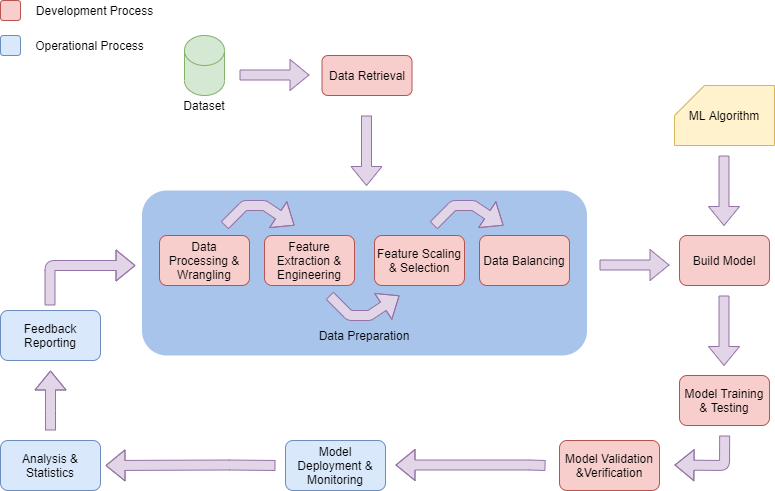
\includegraphics[width=1\textwidth]{figure/Ml Pipeline.png}
        \caption{Esempio generico di pipeline di machine learning basato su MLOps}
\end{figure}
\newpage